% !TeX root = ../main.tex
\section{Results}
\label{sec:results}

% =============================================================================
% Figures already produced are in study/presentation/figures/ and
% study/search_comparison/results_full/ -- reuse them, do not redraw by hand.
% All the numbers below come from the study notes and CSVs; RE-EXTRACT each of
% them from the final results directory before writing, and say which one.
% =============================================================================
% !TeX root = ../main.tex

\add{This section presents the results obtained during the study. We first
give an overview of the complete set of measured configurations and analyse
the distribution of the IO500 SCORE over the search space. We then study
the structure of the response surface and the influence of the different
parameters. The next part compares the search strategies and analyses how
quickly Random Search and Bayesian Optimization find good configurations.
Finally, we compare the different Bayesian Optimization setups and identify
the configuration that gives the best results.}

Figure~\ref{fig:all-results} gives a first overview of all IO500 executions
collected during the exhaustive study. Each point represents one execution
stored in the reference dataset. The SCORE varies strongly across the
different executions, while only a small number of results are close to the
best value found in the dataset.

\begin{figure}[H]
    \centering
    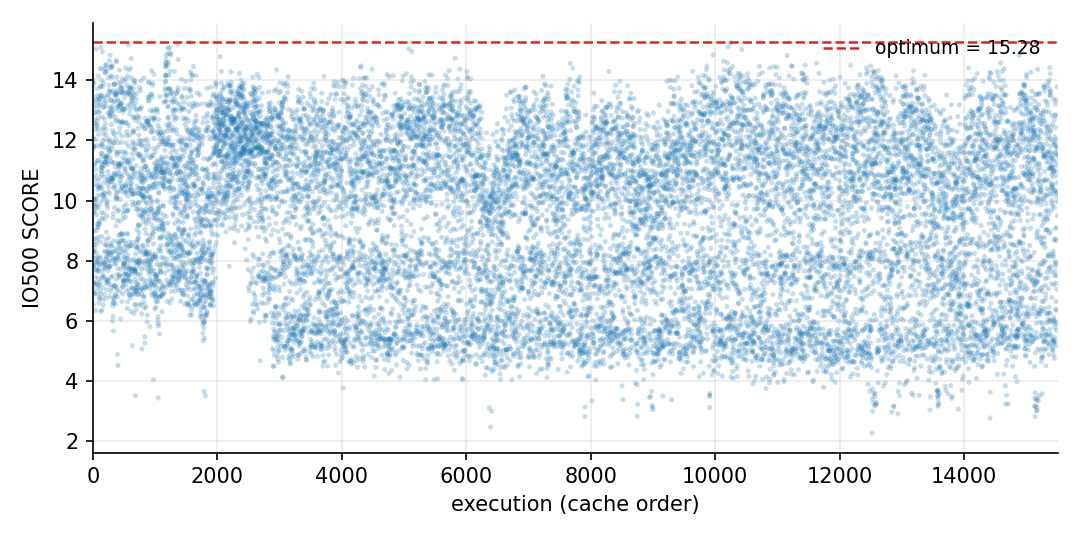
\includegraphics[width=\textwidth]
    {figures/methodology_scatter.png}
    \caption{IO500 SCORE obtained for all executions in the reference
    dataset. The dashed red line shows the best SCORE found, equal to
    approximately 15.28.}
    \label{fig:all-results}
\end{figure}

This first view shows that the parameter space contains configurations with
very different performance levels. The following subsections analyse these
results in more detail.

\subsection{Characterisation of the response surface}

% \begin{itemize}
%     \item Distribution of the SCORE over the whole measured grid: how many
%           configurations are near-optimal, and how heavy is the tail.
%           (\texttt{score\_distribution.csv},
%           \texttt{fig\_score\_distribution.png})
%     \item 2D projections of the response surface
%           (\texttt{fig\_response\_surface\_2d.png}): show that the landscape
%           is neither convex nor separable.
%     \item \textbf{Takeaway to state explicitly}: the optimum is isolated and
%           the surface has interactions, which is why coordinate-wise greedy
%           tuning is structurally at a disadvantage.
% \end{itemize}

Before comparing the different search methods, we first analyse the
structure of the IO500 search space. The objective is to understand how
the SCORE is distributed and whether good configurations are common or
rare.

\paragraph{Distribution of the SCORE.}

Figure~\ref{fig:score-distribution} shows the distribution of the best
SCORE obtained for each configuration. The scores are spread over a wide
range, from values below 7 to a maximum of about 15.28.

The median SCORE is 10.58, and approximately 81\% of the configurations
have a SCORE below 13. This shows that high-performing configurations
represent only a small part of the search space. In particular, the
configurations close to the optimum are much less frequent than
configurations with medium or low scores.

\begin{figure}[H]
    \centering
    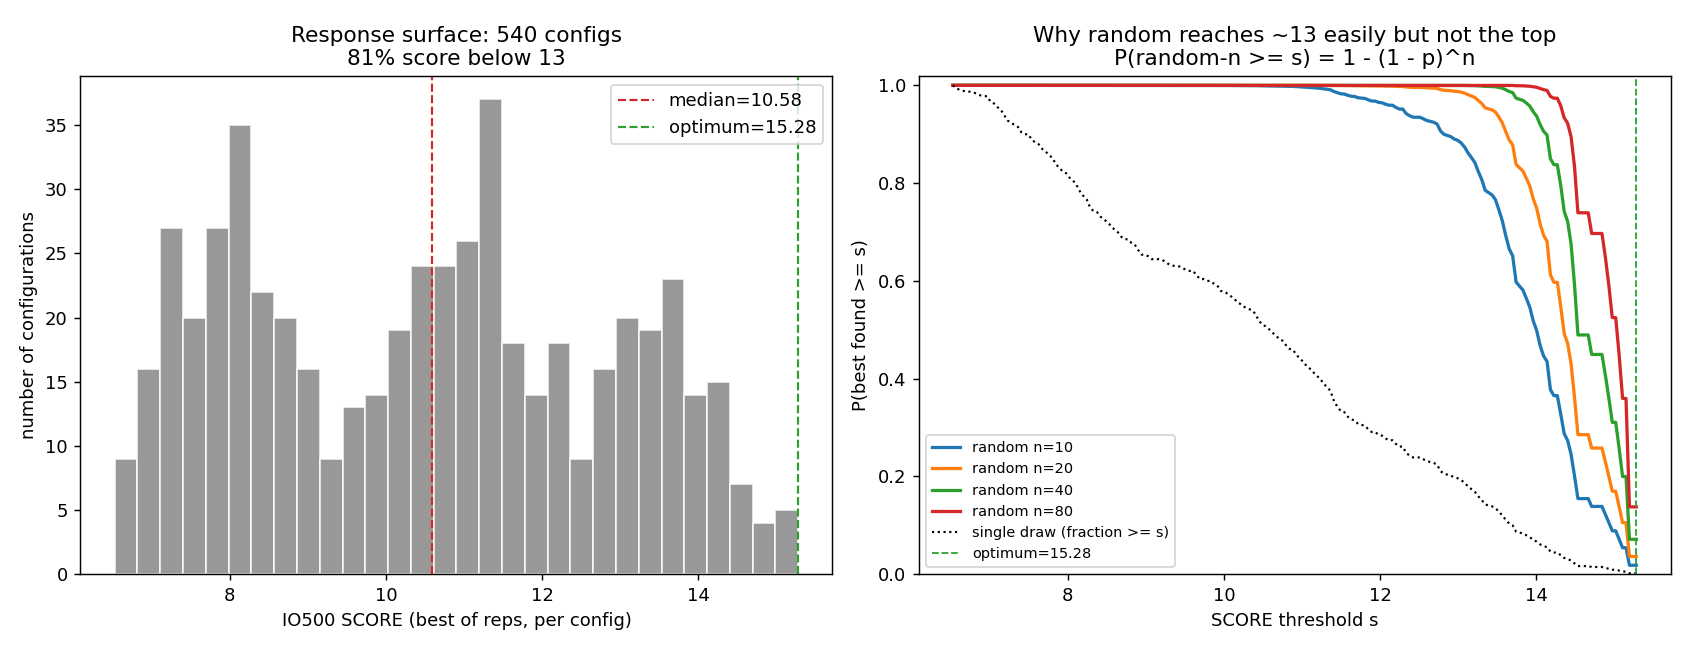
\includegraphics[width=\textwidth]
    {figures/fig_score_distribution.png}
    \caption{Distribution of the IO500 SCORE over the measured
    configurations. The left plot shows the SCORE distribution, while
    the right plot shows the probability of reaching different SCORE
    thresholds with random sampling.}
    \label{fig:score-distribution}
\end{figure}

The distribution has a small upper tail containing the best
configurations. As a result, finding a configuration with a reasonable
SCORE is relatively easy, but finding a configuration very close to the
best SCORE is much more difficult.

The probability curves shown on the right side of
Figure~\ref{fig:score-distribution} illustrate this effect. With a small
number of random evaluations, it is possible to reach medium SCORE
values, while the probability decreases strongly when the target SCORE
approaches the optimum. This result will be discussed in more detail when
analysing Random Search.

\paragraph{Two-dimensional projections.}

The distribution alone does not show how the different parameters affect
the SCORE. To study these effects, Figure~\ref{fig:response-surface}
shows several two-dimensional projections of the response surface.

Each cell represents the mean SCORE obtained for a pair of parameter
values. The other parameters are averaged over the available
configurations. The red star indicates the parameter values of the global
best configuration.

\begin{figure}[H]
    \centering
    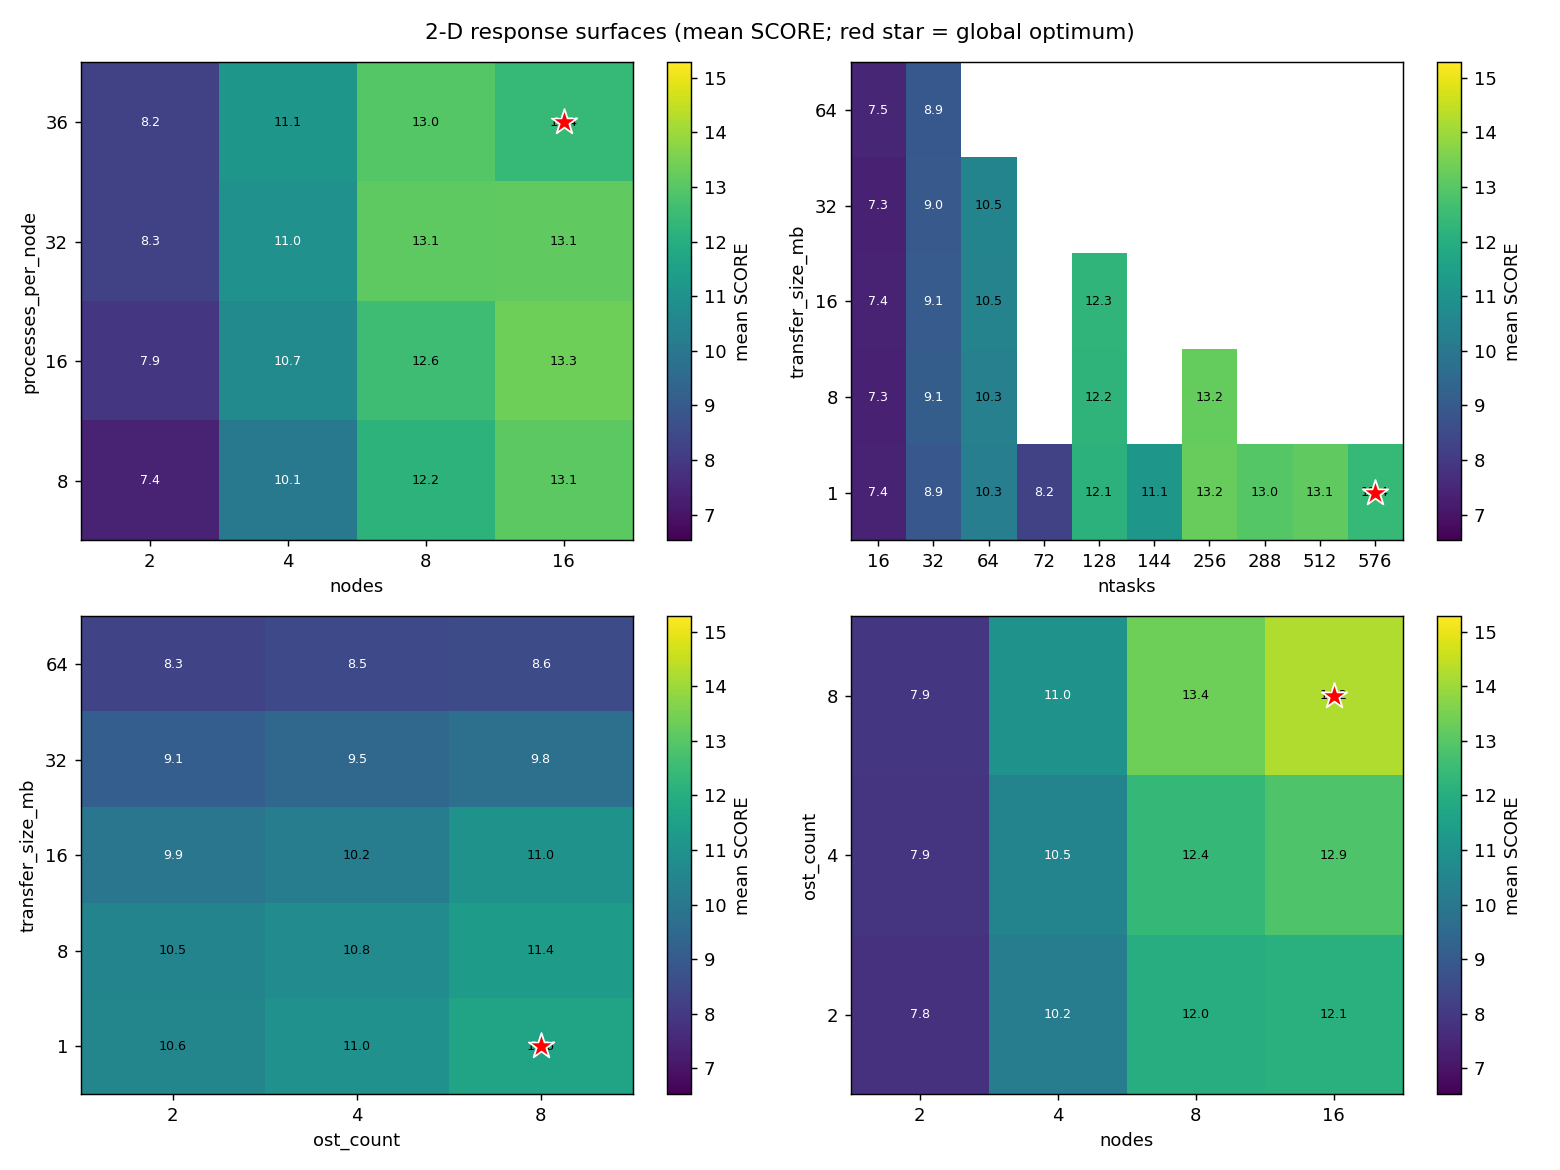
\includegraphics[width=\textwidth]
    {figures/fig_response_surface_2d.png}
    \caption{Two-dimensional projections of the IO500 response surface.
    Each cell shows the mean SCORE for a pair of parameter values. The
    red star indicates the global optimum.}
    \label{fig:response-surface}
\end{figure}

Several trends can be observed. Increasing the number of nodes generally
improves the SCORE, but the effect of the number of processes per node
depends on the number of nodes. This means that the two parameters
interact and should not be considered independently.

A similar behaviour can be observed for the transfer size. Its effect
depends on the total number of tasks and on the number of storage targets.
For example, increasing the number of storage targets has only a small
effect for some transfer sizes, while the improvement is much larger for
others.

The projection between the number of nodes and the number of storage
targets also shows that higher values of both parameters generally lead
to better scores. The best configuration is located in a small region
with a high number of nodes and storage targets.

Overall, the response surface does not behave like a simple convex or
separable function. The effect of one parameter can change depending on
the values of the other parameters. This confirms that parameter
interactions are important in IO500 tuning.

\paragraph{Main observation.}

The two analyses lead to the same conclusion. First, configurations close
to the optimum are rare. Second, the parameters interact with each other,
and the best value of one parameter can depend on the values of the
others.

This makes one-parameter-at-a-time tuning difficult. A method that changes
one parameter while keeping all the others fixed can find a good local
choice but can miss better combinations of parameters. This motivates
the use of search methods that explore several parameters together.

\subsection{Which Bayesian Optimization setup wins?}
% \begin{itemize}
%     \item Ranking of the 83 BO configurations
%           (\texttt{best\_setup\_ranking.png}).
%     \item \textbf{Main finding: the surrogate matters most -- the top-5 setups
%           are all Gaussian Process.} Acquisition (LCB vs EI) is close to a tie
%           at the top.
%     \item Sensitivity analysis, one knob at a time: rank the influence of
%           estimator, acquisition, $\xi$/$\kappa$ and $n_{\text{initial}}$.
%     \item Practical recommendation for a practitioner who will run this once:
%           state a single default tuple (surrogate, acquisition, exploration,
%           $n_{\text{initial}}$) and justify it.
% \end{itemize}
To determine which combination works best for IO500, the different
Bayesian Optimization setups were compared using their mean best SCORE
over the considered budgets. Figure~\ref{fig:best-bo-ranking} shows the
ranking of the best-performing setups.
\begin{figure}[H]
    \centering
    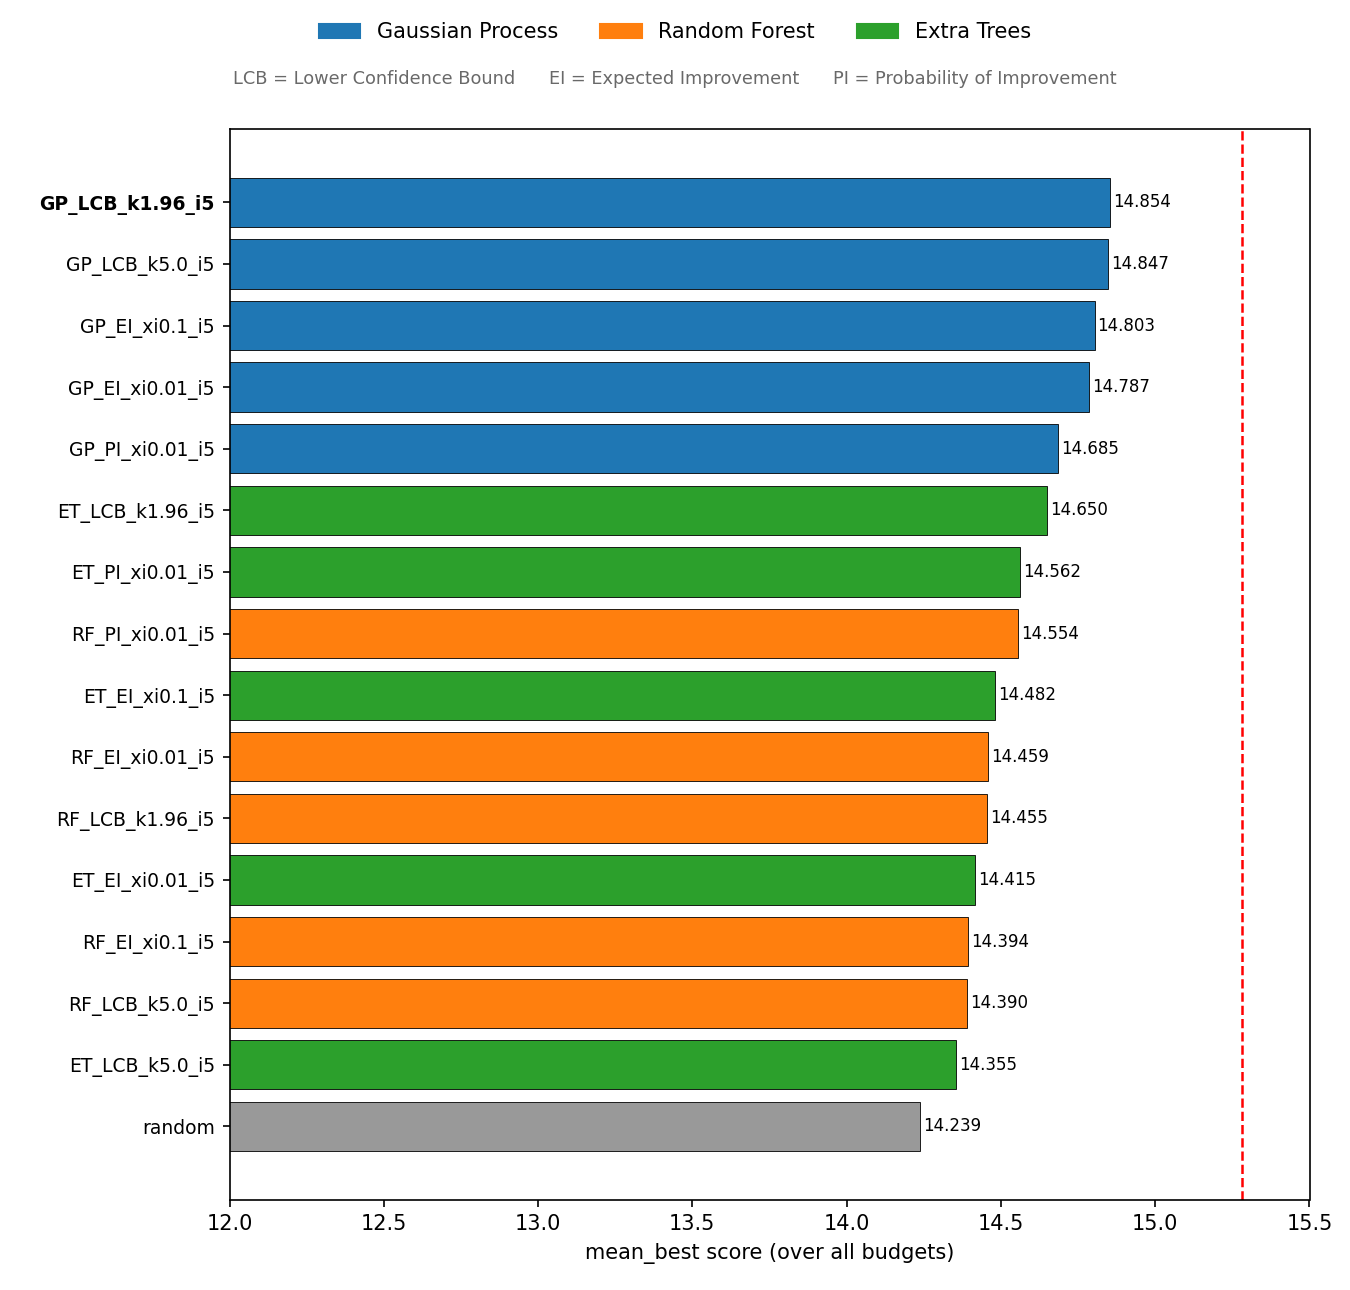
\includegraphics[width=\textwidth]
    {figures/best_setup_ranking.png}
    \caption{Ranking of the best Bayesian Optimization setups according
    to their mean best IO500 SCORE. The dashed red line represents the
    global optimum of the reference dataset.}
    \label{fig:best-bo-ranking}
\end{figure}

\paragraph{Influence of the surrogate model.}

The clearest result is the influence of the surrogate model. The
best-performing setups in Figure~\ref{fig:best-bo-ranking} all use a
Gaussian Process (GP).

The best setup is \texttt{GP\_LCB\_k1.96\_i5}, with a mean best SCORE of
14.854. It is followed closely by \texttt{GP\_LCB\_k5.0\_i5}, with a
SCORE of 14.847. Other high-ranking setups also use a Gaussian Process
combined with EI or PI.

The best setups based on Extra Trees and Random Forest obtain lower
scores. This suggests that the surrogate model has a strong effect on the
quality of the search. Among the models considered in this study,
Gaussian Process gives the best results.

\paragraph{Influence of the acquisition function.}

The acquisition function also affects the results, but the difference
between the best acquisition functions is smaller.

LCB gives the two highest scores. However, EI is very close. For example,
the best LCB setup reaches 14.854, while the best EI setup reaches
14.803.

This shows that both LCB and EI work well when combined with a Gaussian
Process. PI also gives good results, but it remains slightly below the
best LCB and EI setups.

The results therefore suggest that choosing the surrogate model is more
important than choosing between LCB and EI.

\paragraph{Influence of the exploration parameter.}

The exploration parameter controls the balance between testing regions
that already look promising and exploring less-known parts of the
parameter space.

For LCB, this behaviour is controlled by \texttt{kappa}. The setups with
\texttt{kappa = 1.96} and \texttt{kappa = 5.0} obtain very similar
results.

For EI, the parameter \texttt{xi} controls exploration. The results with
\texttt{xi = 0.1} and \texttt{xi = 0.01} are also close.

This indicates that the exact value of the exploration parameter has a
smaller influence on the final result than the choice of surrogate model.

These initial points provide the first observations used to build the
surrogate model before the guided search starts. The results suggest that
five initial points provide a good balance between collecting initial
information and leaving enough evaluations for the guided part of the
search.

\paragraph{Practical recommendation.}

Based on these results, the following configuration is selected as the
default Bayesian Optimization setup:

\begin{minted}[
    fontsize=\small,
    frame=lines,
    breaklines=true
]{yaml}
bayesian_config:
  objective_metric: "SCORE"
  objective: "maximize"
  n_initial_points: 5
  acquisition_func: "LCB"
  base_estimator: "GP"
  kappa: 1.96
\end{minted}

This setup gives the highest mean best SCORE in the comparison. It
therefore provides a simple default for a user who wants to apply
Bayesian Optimization to IO500 without having to compare many different
settings.

Overall, the results show that the surrogate model has the strongest
visible influence on performance. Gaussian Process performs best, while
the difference between LCB and EI is much smaller. The recommended
configuration is therefore a Gaussian Process with LCB,
\texttt{kappa = 1.96}, and five initial points.

\subsection{Why random search is not enough}

% \begin{itemize}
%     \item Analytic argument from the measured score distribution: reaching
%           SCORE $\geq$ 15 with 90\,\% probability by chance requires
%           $\approx 1{,}081$ tests.
%     \item \textbf{Takeaway}: the near-optimal tail is effectively unreachable
%           by luck; random search is a good baseline for \emph{average}
%           quality and a bad strategy for \emph{peak} quality.
%     \item Nuance to keep (it is honest and it strengthens the report): at very
%           low budgets, random is competitive with, and sometimes better than,
%           the tree-based surrogates.
% \end{itemize}


Random Search can find reasonable configurations with a small number of
evaluations. However, the distribution of the measured IO500 scores shows
that configurations close to the optimum are very rare.

This can be analysed directly from the exhaustive reference dataset. If
$p$ is the fraction of configurations that reach a given SCORE threshold,
the probability of finding at least one of them after $n$ random
evaluations is:

\[
P = 1 - (1-p)^n.
\]

This probability can be used to estimate how many random evaluations are
needed to reach a target SCORE with a given confidence.

For moderate SCORE values, Random Search needs only a small number of
evaluations. However, the required number increases quickly when the
target approaches the optimum. In particular, reaching a SCORE of at
least 15 with a probability of 90\% requires approximately 1,081 random
evaluations.

This large number comes from the fact that very few configurations in the
reference dataset reach this level. Therefore, randomly selecting one of
these near-optimal configurations is unlikely when the evaluation budget
is small.

This does not mean that Random Search always performs poorly. With very
small budgets, it can be competitive with some Bayesian Optimization
configurations and can sometimes perform better than methods based on
tree surrogate models. Random Search is therefore a useful baseline and
can find configurations with reasonable performance quickly.

Its main limitation appears when the objective is to find a configuration
very close to the optimum. In this case, the high-scoring region is too
small to be reached reliably by chance. Random Search is therefore more
suitable for finding an acceptable configuration than for finding the
best configurations in the search space.

This result motivates the use of a guided search method. Instead of
sampling configurations independently, Bayesian Optimization uses the
results already observed to direct the search toward more promising parts
of the parameter space.


\subsection{Automated search versus a human specialist}

% \begin{itemize}
%     \item Protocol recap and the specialist's submitted candidates.
%     \item \textbf{Result: the expert's best informed pick reached
%           $\approx$ 95\,\% of the optimum; BO with 40 evaluations reached
%           $\approx$ 98\,\%} (\texttt{specialist\_vs\_bo.png}).
%     \item Discuss fairly: the expert answered in minutes and without access to
%           the machine's response surface; the interesting claim is not ``the
%           machine beats the human'' but ``a modest automated budget matches or
%           exceeds expert intuition, reproducibly''.
%     \item Limitation to state: only one specialist has submitted so far, so
%           this is an illustration, not a statistically meaningful comparison.
% \end{itemize}

To complement the comparison between search algorithms, the automated
methods were also compared with a configuration proposed by a human
specialist.

The specialist submitted three configurations based on experience and
knowledge of IO500 and HPC storage systems. No exhaustive information
about the response surface was available when these configurations were
chosen.

Figure~\ref{fig:specialist-vs-bo} compares the best specialist
configuration with Random Search and Bayesian Optimization.

\begin{figure}[H]
    \centering
    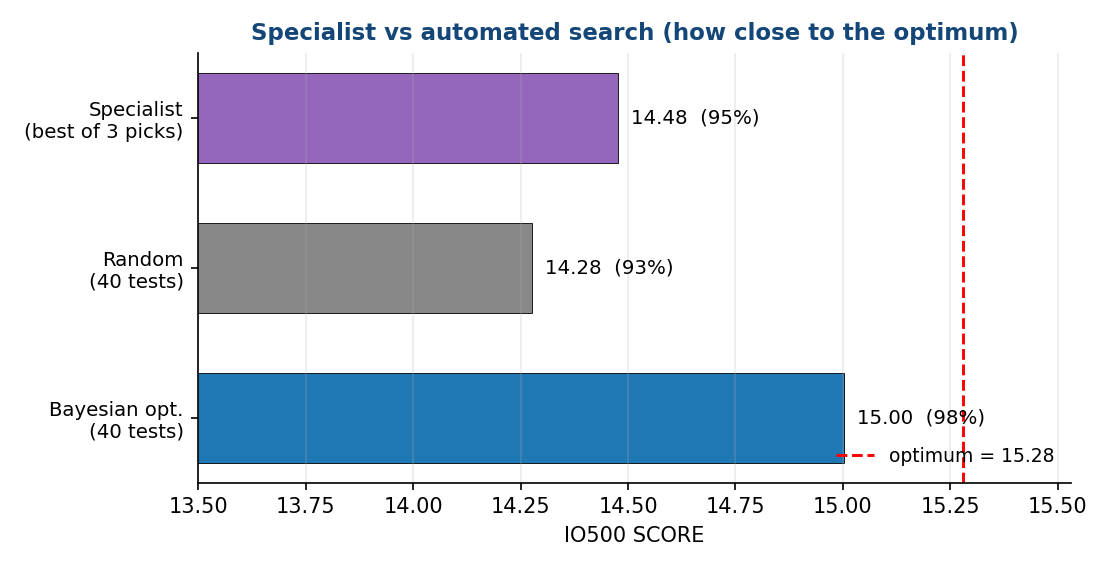
\includegraphics[width=0.9\textwidth]
    {figures/specialist_vs_bo.png}
    \caption{Comparison between the best configuration proposed by a
    specialist, Random Search with 40 evaluations, and Bayesian
    Optimization with 40 evaluations. The dashed red line represents the
    optimum of the reference dataset.}
    \label{fig:specialist-vs-bo}
\end{figure}

The best configuration proposed by the specialist obtained a SCORE of
14.48, which corresponds to approximately 95\% of the optimum SCORE of
15.28. This shows that expert knowledge can identify a very good
configuration without exploring a large part of the parameter space.

Random Search with 40 evaluations reached a SCORE of 14.28, or about
93\% of the optimum. Bayesian Optimization with the same budget of 40
evaluations reached a SCORE of 15.00, corresponding to approximately
98\% of the optimum.

The important result is not that the automated method ``beats'' the
specialist. The specialist selected the configurations in a short amount
of time and without access to the complete measured response surface. In
contrast, Bayesian Optimization uses several evaluations and learns from
the results obtained during the search.

The comparison instead shows that, with a relatively small evaluation
budget, Bayesian Optimization can reach or exceed the quality of an
expert-informed configuration in a systematic and reproducible way.

This result should nevertheless be interpreted with care. Only one
specialist participated in this experiment and only three configurations
were submitted. The comparison is therefore an illustration rather than
a statistically meaningful evaluation of human expertise.
\subsection{Example of a proposed comparison between valid and invalid IO500
scores}
\label{sec:proposed-validation}

The reduced-cost IO500 executions were introduced as a possible way to
explore the parameter space faster. However, this approach was not fully
validated during the internship.

A possible validation experiment would be to compare valid and invalid
IO500 executions using the same parameter values. 

The number of storage targets could then be varied from 1 to 8. Several
repetitions could be performed for each value using both valid and
reduced-cost IO500 settings.

Figure~\ref{fig:valid-invalid-ost} illustrates the type of comparison that
could be used for this validation.

\begin{figure}[H]
    \centering
    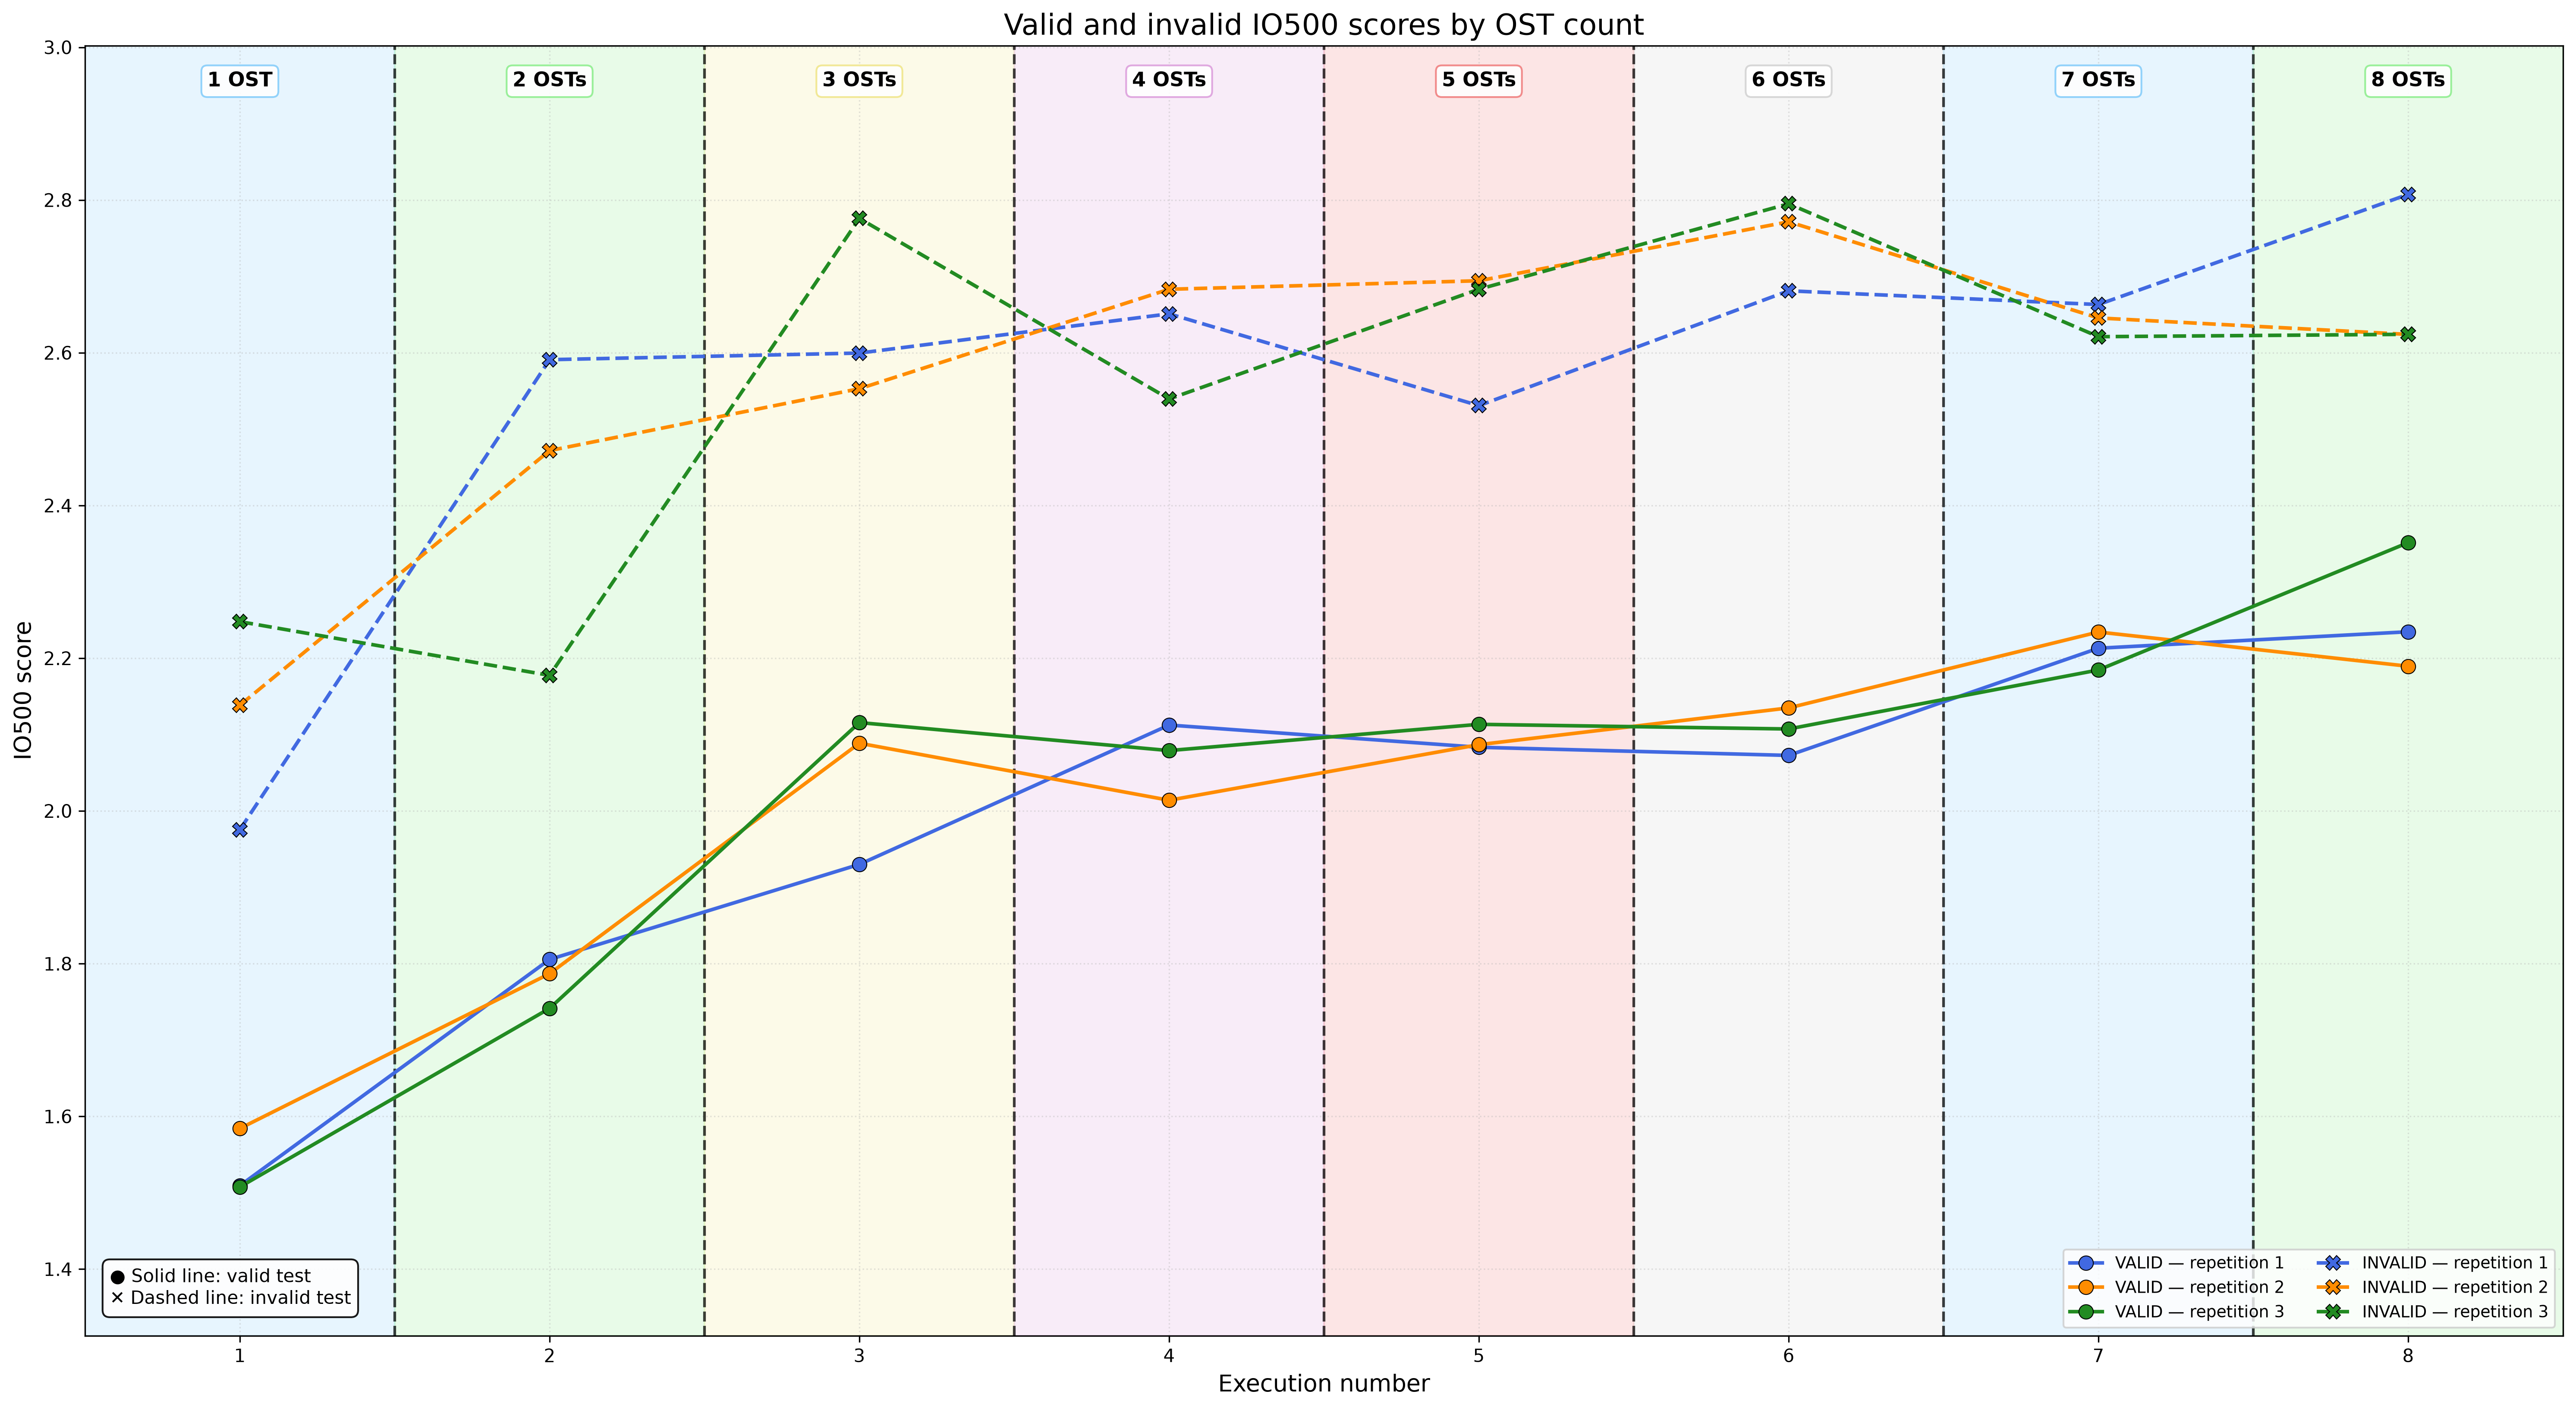
\includegraphics[width=\textwidth]
    {figures/OTSI_valid_invalid_scores_by_ost.png}
    \caption{Example of a possible comparison between valid and invalid
    IO500 scores when varying the number of storage targets.}
    \label{fig:valid-invalid-ost}
\end{figure}

The goal of such an experiment would not be to convert an invalid SCORE
into a valid SCORE. Instead, it would be to study whether the relative
behaviour of the configurations is similar in both cases.

If similar trends are observed, reduced-cost executions could be useful
for guiding the search before validating the final configurations with
official IO500 runs. If the trends are very different, the reduced-cost
approach would not be reliable enough for this purpose.

This validation was not completed during the internship and is therefore
left as future work.


\subsection{IOPS: IO500 support and new optimization methods}
\label{sec:iops-extensions}

As the internship progressed, the work was extended to the development of
IOPS. In addition to using IOPS to run the experiments, new features were
added to make IO500 easier to configure and to extend the available
optimization methods.

The first contribution was the addition of IO500 support in IOPS. The
second contribution was the implementation of the Tree-structured Parzen
Estimator (TPE) as a new search method. The IOPS documentation was also
updated to describe these new features and explain how they can be used.


\subsubsection{IO500 plugin in IOPS}
\label{sec:iops-io500-plugin}

Before this work, an IO500 experiment had to be configured manually in
IOPS. During the internship, an IO500 plugin was added to simplify this
process.

The plugin allows the user to generate an IO500 configuration template
with a simple command:


\begin{minted}[
    fontsize=\small,
    frame=lines,
    breaklines=true,
    bgcolor=gray!5,
    escapeinside=||
]{text}
|\textcolor{blue}{iops}| |\textcolor{teal}{generate}| |\textcolor{red}{--io500}|
\end{minted}
When this command is executed, IOPS generates a YAML configuration file
that contains the main elements needed to run an IO500 experiment. The
generated file can then be modified according to the target machine,
storage system, and experiment.

Figure~\ref{fig:iops-generate-io500} shows an example of the command used
to generate the configuration.

\begin{figure}[H]
    \centering
    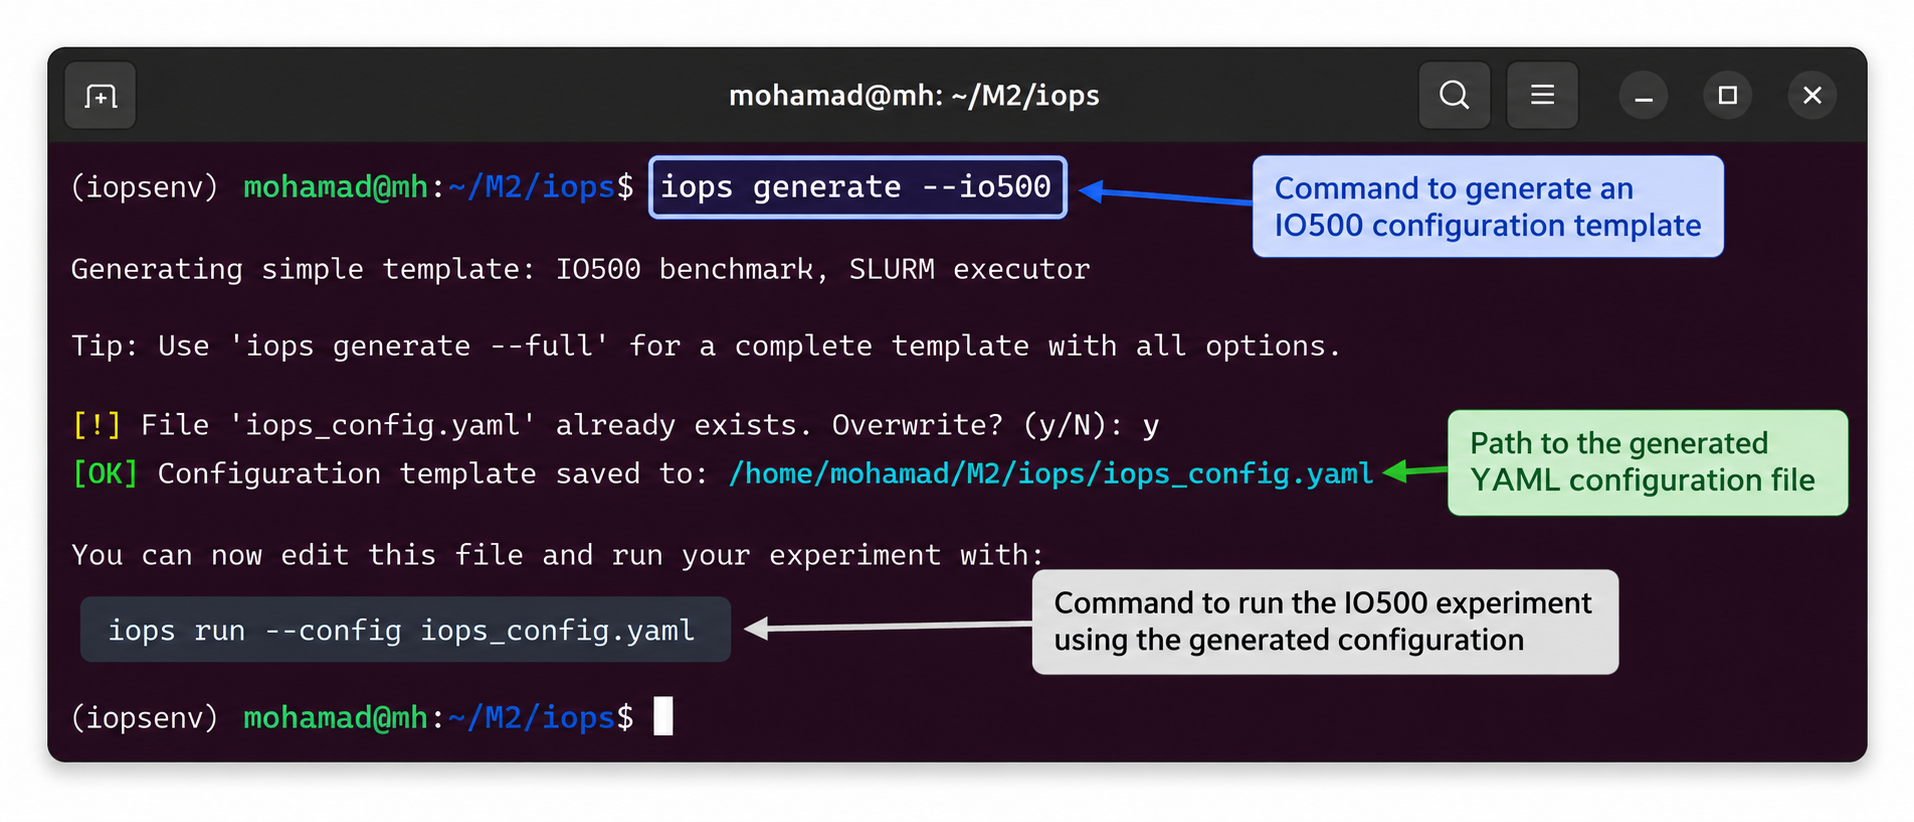
\includegraphics[width=0.9\textwidth]
    {figures/iops_generate_io500.png}
    \caption{Generation of an IO500 configuration template with IOPS.}
    \label{fig:iops-generate-io500}
\end{figure}

The generated YAML file includes the main parameters that can be adapted
by the user. These include the number of compute nodes, the number of MPI
processes per node, the total number of MPI tasks, the dataset size, the
transfer size, the block size, the segment count, the number of storage
targets, and the file organization parameters.

Some parameters are selected directly by the user, while others can be
computed automatically. For example, the total number of MPI tasks can
be calculated from the number of nodes and the number of processes per
node.

The generated configuration is intended to be a starting point rather
than a fixed configuration. The user should adapt it to the HPC platform
and storage system before running the benchmark.

The documentation of IOPS was also updated to explain how to use this new
functionality. It describes the command used to generate the template and
the main parameters that should be adapted.

Figure~\ref{fig:iops-io500-documentation} shows part of the documentation
added for the IO500 plugin.

\begin{figure}[H]
    \centering
    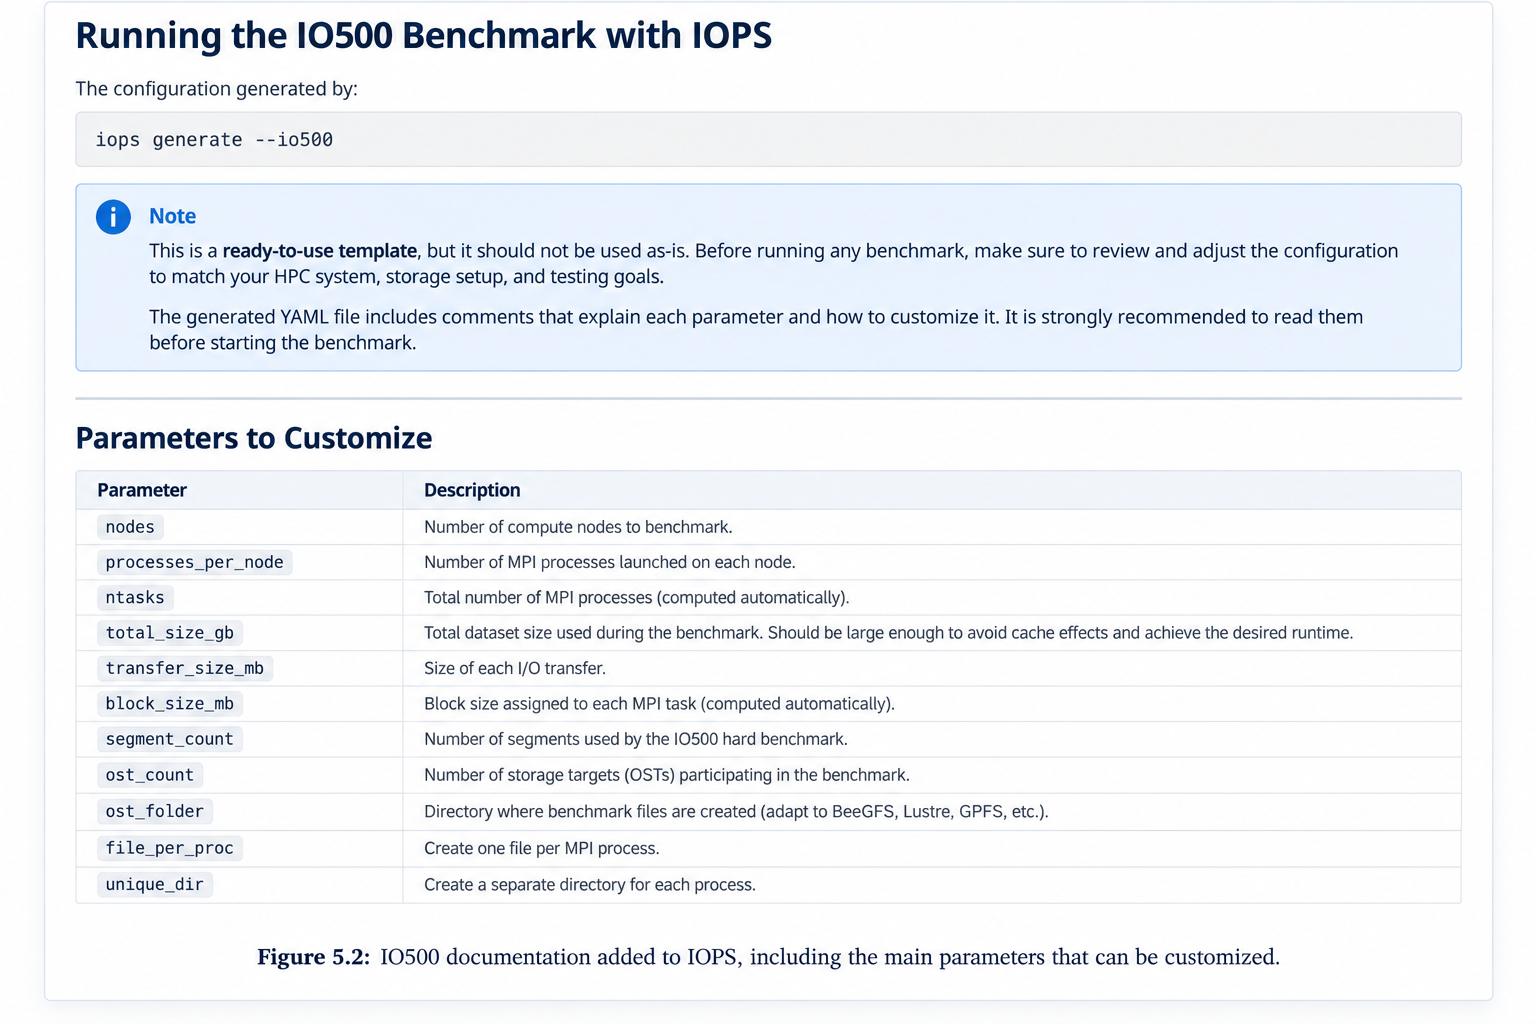
\includegraphics[width=\textwidth]
    {figures/iops_io500_documentation.png}
    \caption{IO500 documentation added to IOPS.}
    \label{fig:iops-io500-documentation}
\end{figure}

This contribution provides a simpler and more reproducible way to prepare
IO500 experiments. A user can generate a template, modify the required
parameters, and use the resulting YAML file directly with IOPS.


\subsubsection{Tree-structured Parzen Estimator}
\label{sec:iops-tpe}

The search component of IOPS was also extended during the internship.
The Tree-structured Parzen Estimator (TPE) was implemented as an
additional optimization method.

TPE is a guided optimization method that uses the results of previous
evaluations to choose new configurations. In this sense, its objective is
similar to Bayesian Optimization: both methods try to avoid testing the
complete parameter space and use previous observations to guide the
search.

However, the two approaches build their models differently.

Bayesian Optimization builds a surrogate model that estimates the
objective function. In this study, the objective function represents the
relation between a configuration and its IO500 SCORE. Based on this
model, an acquisition function is used to select the next configuration
to evaluate.

TPE uses another approach. Instead of directly predicting the SCORE, it
uses the previous observations to separate configurations according to
their performance. It models the distribution of parameter values for
good configurations and compares it with the distribution of
lower-performing configurations.

The general idea can be represented as:

\[
\text{previous evaluations}
\rightarrow
\text{separate good and lower-performing configurations}
\rightarrow
\text{model their parameter distributions}
\rightarrow
\text{select a promising configuration}.
\]

Figure~\ref{fig:bo-vs-tpe} illustrates the main difference between
Bayesian Optimization and TPE.

\begin{figure}[H]
    \centering
    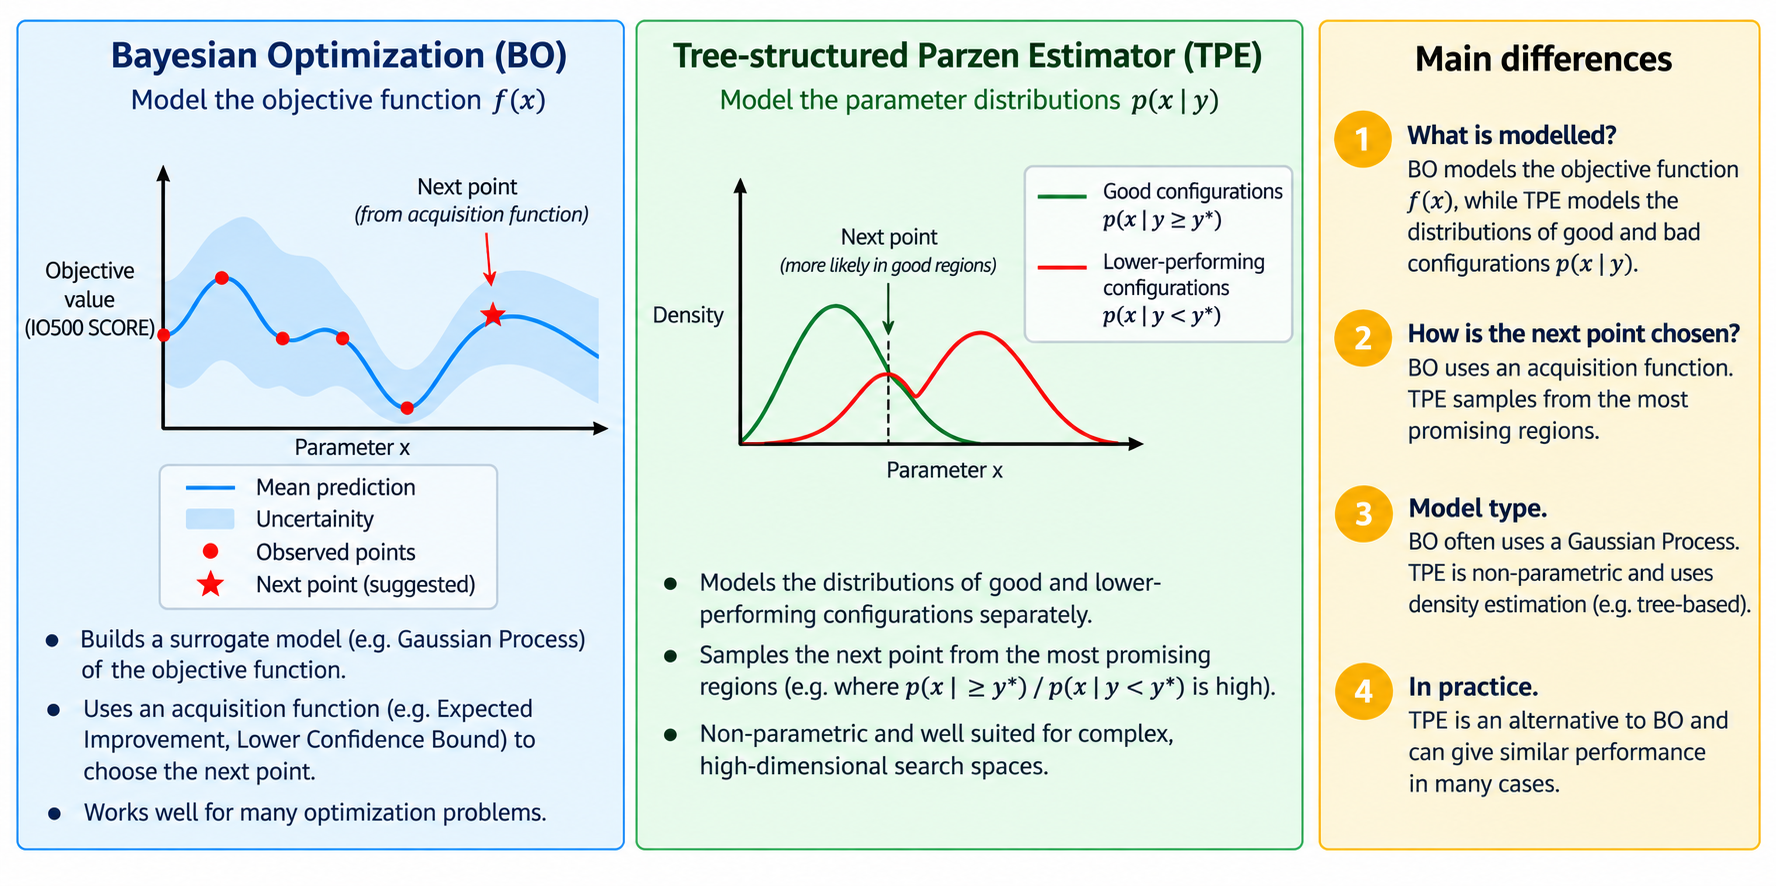
\includegraphics[width=\textwidth]
    {figures/bo_vs_tpe.png}
    \caption{Simplified comparison between Bayesian Optimization and
    TPE. Bayesian Optimization models the objective function, while TPE
    models the parameter distributions of good and lower-performing
    configurations.}
    \label{fig:bo-vs-tpe}
\end{figure}

Both methods therefore use previous results to guide the search, but they
use this information differently. Bayesian Optimization predicts the
performance of configurations using a surrogate model and an acquisition
function, while TPE searches for parameter values that appear more often
in the group of good configurations.

The TPE method was implemented in IOPS during the internship. However, it
was not evaluated on the IO500 experiments. It is therefore presented as
a software contribution rather than as one of the methods included in the
experimental comparison of this report.

Other optimization methods were also considered as possible future
extensions. These include Iterated Racing (irace) and the Covariance
Matrix Adaptation Evolution Strategy (CMA-ES). These methods were
considered during the internship but were not included in the experimental
evaluation.

These developments extended the initial scope of the internship and
contributed to making IOPS easier to use for IO500 experiments and easier
to extend with new search methods.

